\chapter{Разработка расчетной сетки и аппроксимация свойств местности на узлы сетки}
\label{chap_mesh}

\section{Расчетная сетка в методе конечных элементов}
\label{sec_fin_elem_mesh}

Для решения уравнения адвекции-диффузии, описанного в разделе \ref{diffusion_model}, в модели \ac{ascro} применяется 
метод конечных элементов. В этом методе область, в которой ищется решение уравнения, разбивается на конечное количество 
подоблостей. Каждая из этих подобластей называется элементами. В каждом элементе выбирается вид аппроксимирующей функции. 
Вне своего элемента аппроксимирующая функция равняется нулю. Значения функций в узлах элементов заранее неизвестны и 
являются решением задачи. Вначале ищутся коэффициенты аппроксимирующих функций из условия равенства соседних функций в 
узлах элементов. После этого, коэффициенты выражаются через значения функций в узлах элементов. Составляется система 
линейных алгебраических уравнений, количество уравнений в которой равно количеству неизвестных значений в узлах, в 
которых ищется решение системы. 

Расчетная сетка в модели \ac{ascro} имеет форму цилиндра и представляет собой участок местности вблизи \ac{aes}. 
Так как расчетная сетка имеет форму цилиндра, её элементы должны быть трехмерными.

Существует четыре основных типа трехмерных элементов: тетраэдры, гексаэдры, призмы и пирамиды (рисунок 
\ref{fig_finite_elements}). Самым распространенным элементом при построении расчетных сеток являются тетраэдры. 

\begin{figure}[ht]
\centering
	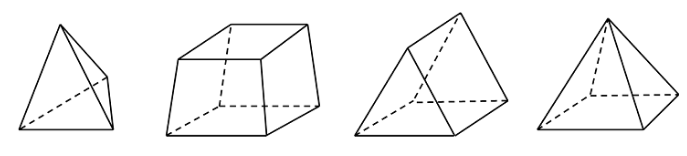
\includegraphics[width=16cm]{finite_elements}
	\captionsetup{justification=centering}
    \caption{Основные типы трехмерных элементов расчетной сетки.}
    \label{fig_finite_elements}
\end{figure}

Тетраэдрический элемент является простейшим элементом и позволяет построить расчетную сетку практически для любого 
трёхмерного тела. В модели \ac{ascro} для решения уравнения адвекции-диффузии методом конечных элементов используется 
расчетная сетка с тетраэдрическими элементами.

\section{Создание расчетной сетки}
\label{sec_mesh_gen}

Построение расчетной сетки для решении уравнения методом конечных элементов является сложной задачей, особенно для 
объекта нетривиальной формы. Как правило, создание расчетных сеток представляет собой трудоемкий и кропотливый процесс. 
В современном мире существует ряд технологий, позволяющих упростить создание расчетной сетки: программа \textit{gmsh}, 
предназначенная для построения трёхмерных расчетных сеток для решения задач методом конечных элементов \cite{gmsh_man}, 
а так же библиотека \textit{pygmsh} для языка программирования Python \cite{pygmsh_doc}, предоставляющая удобный 
интерфейс для работы с программой \textit{gmsh}.

Как было отмечено в разделе \ref{sec_fin_elem_mesh}, расчетная сетка в проекте \ac{ascro} имеет цилиндрическую форму. 
Программный модуль, который отвечает за создание расчетной сетки, должен принимать в качестве входных данных такие 
параметры, как: высота рассматриваемой области в метрах, радиус рассматриваемой области в метрах и шаг между соседними 
узлами расчетной сетки.

Важной задачей является выбор шага между узлами расчетной сетки. Согласно \cite{mke}, точность решения уравнения методом 
конечных элементов во многом зависит от качества разбиения исходной области на конечные элементы и от числа узлов 
конечных элементов. Таким образом, чем гуще расчетная сетка, тем ближе решение, полученное численным методом конечных 
элементов, к аналитическому решению. 

Так как радиус рассматриваемой области планируется делать порядка 30 км вокруг источника выброса радиоактивных примесей 
(вокруг \ac{aes}), делать сетку одинаково большой точности на всей рассматриваемой области не эффективно с точки зрения 
вычислительных мощностей \ac{evm} (\acl{evm}). Более того, расчет распространения радиоактивных примесей планируется 
проводить в реальном времени, что накладывает ограничение на время расчета. 

В связи с поставленными выше ограничениями, было решено сделать различную густоту расчетной сетки при удалении от 
источника радиоактивных выбросов. Расчетная сетка должна быть достаточно детальной вблизи \ac{aes} и по мере удаленности 
от источника радиоактивных выбрасов становиться более разряженной. Следовательно, шаг расчетной сетки должен меняться.

В итоге, в соответствии с поставленными выше требованиями, был разработан программный модуль генерации расчетной сетки. 
Схема разработанного модуля представлена на рисунке \ref{fig_mesh_gen_scheme}. 

\begin{figure}[ht]
	\centering
	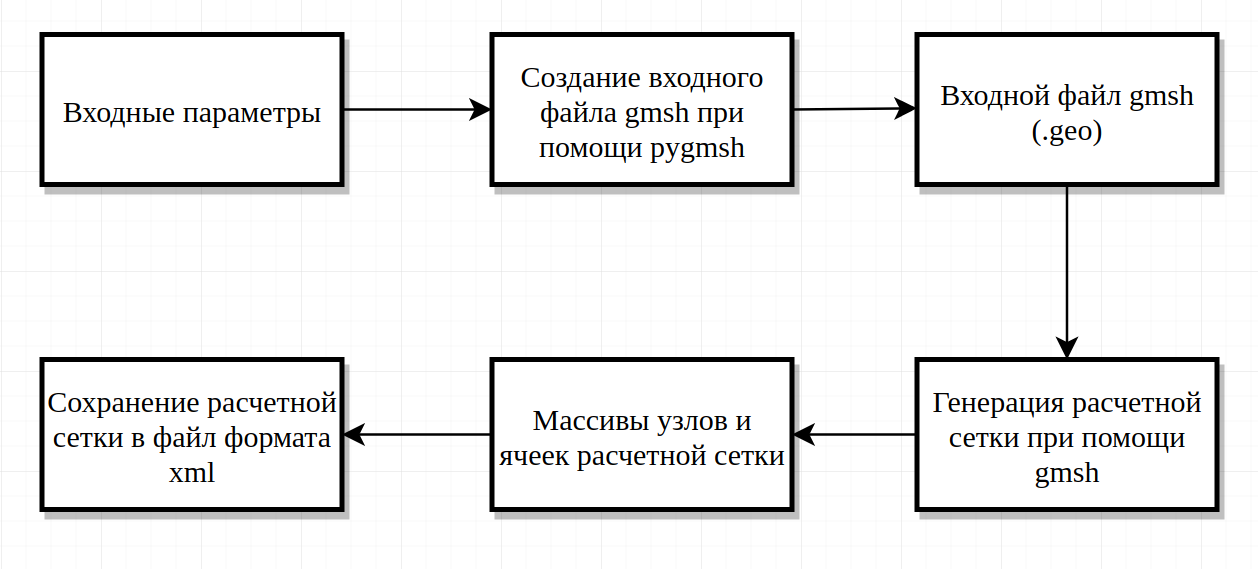
\includegraphics[width=16cm]{mesh_gen_scheme}
	\captionsetup{justification=centering}
    \caption{Схема модуля генерации расчетной сетки.}
    \label{fig_mesh_gen_scheme}
\end{figure}

На вход модуль принимает следующие параметры, необходимые для создания расчетной сетки: высота и радиус рассматриваемой 
области вблизи \ac{aes}; список радиусов, для которых будет задан шаг расчетной сетки; список шагов расчетной сетки для 
каждой области из списка радиусов. Входные параметры задаются в конфигурационном файле проекта.

На втором шаге входные параметры программно считываются при помощи языка программирования Python и на их основе 
происходит процесс создания входного файла для программы \textit{gmsh}. Для создания входного файла используется 
библиотека \textit{pygmsh}, которая позволяет при помощи удобных абстракций задать необходимую геометрию расчетной сетки 
и на основе полученной геометрии сгенерировать файл, содержащий команды на скриптовом языке \textit{gmsh}, в котором 
детально описываются опорные точки и линии создаваемой геометрии. 

Далее, полученный скриптовый файл с расширением \textit{.geo} передается входным параметром программе \textit{gmsh}, 
которая в свою очередь генерирует расчетную сетку. На выходе программа выдает массив, содержащий информацию об узлах и 
ячейках построенной расчетной сетки.

В дальнейшем, для численного решения уравнения адвекции-диффузии методом конечных элементов будет использоваться 
вычислительный пакет \textit{FEniCS}, который требует, чтобы файл расчетной сетки имел формат \textit{xml}. Для этого, 
в модуле генерации расчетной сетки присутствует последний шаг, выполняющий сохранение полученных массивов узлов и ячеек 
сетки в файл формата \textit{xml}.

Пример построенной расчетной сетки при помощи вышеописанного модуля представлен на рисунке \ref{fig_mesh_img}.

\begin{figure}[ht]
	\centering
	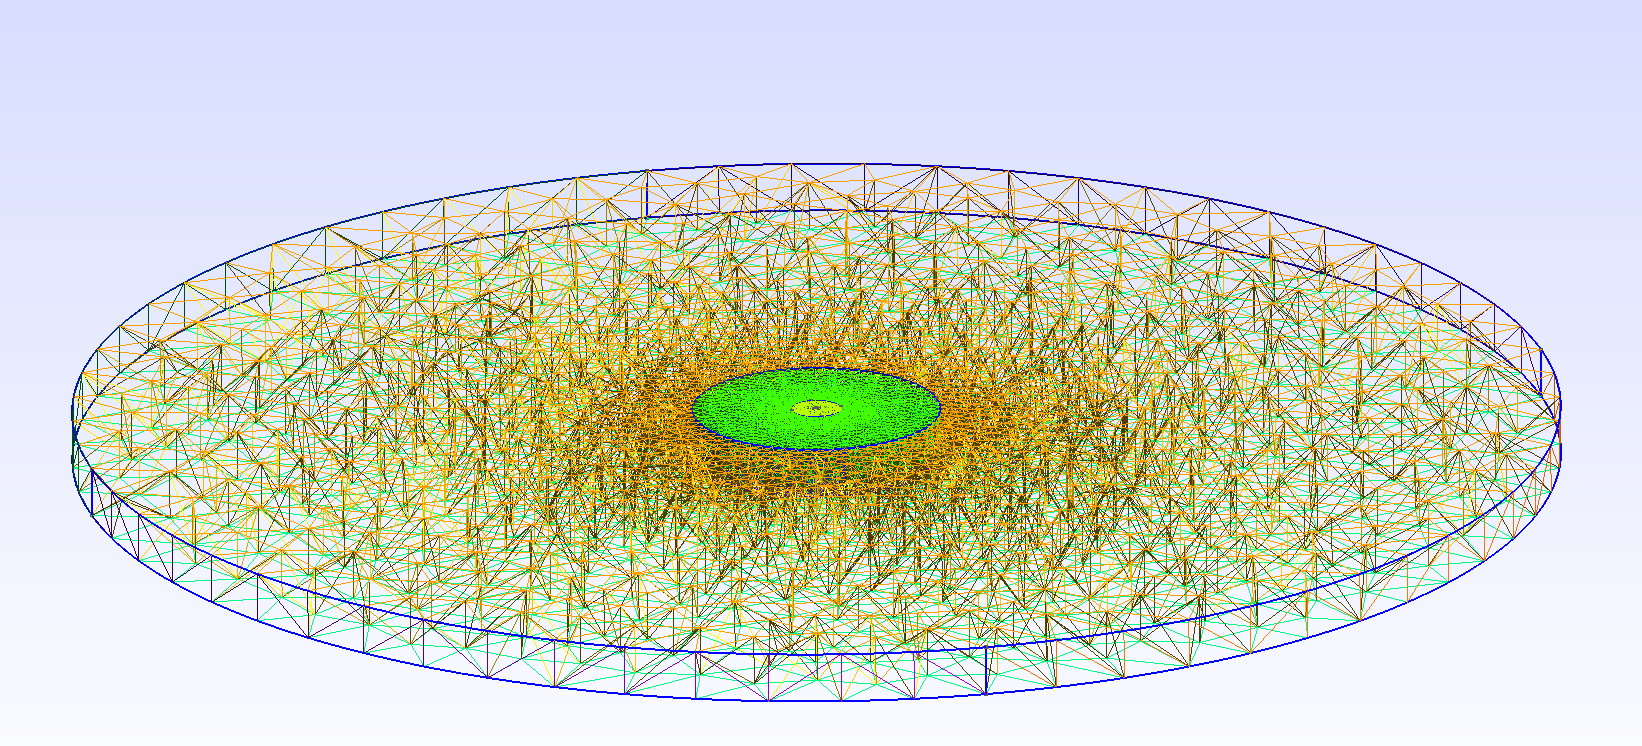
\includegraphics[width=16cm]{mesh}
	\captionsetup{justification=centering}
    \caption{Расчетная сетка, построенная при помощи разработанного модуля.}
    \label{fig_mesh_img}
\end{figure}

\section{Аппроксимация свойств местности на узлы расчетной сетки}

Ранее в главе \ref{chapter_surf_type} был проведен анализ топологической карты местности вблизи \ac{aes} и получена 
информация о каждом из пикселей топологической карты. Текущей задачей является создание модуля аппроксимации свойств 
местности на узлы расчетной сетки, разработанной в разделе \ref{sec_mesh_gen}, для последующего решения уравнения 
адвекции-диффузии.

Для начала необходимо определить соответствие координат узлов расчетной сетки и индексов пикселей в массиве, полученном 
в разделе \ref{sec_mesh_gen}. Для этого была разработана функция, которая определяет такое соответствие согласно формуле 
\ref{eq_coords_to_pix}.

\begin{equation}
    \label{eq_coords_to_pix}
	k_i = \frac{x_i+r}{2 \times r / s_i}    
\end{equation}

где:
\begin{description}
    \item $k_i$ --- индекс пикселя в продольном или поперечном направлении;
    \item $x_i$ --- продольная или поперечная координата (м);
    \item $r$ --- радиус рассматриваемой прилегающей к \ac{aes} местности (м);
    \item $s_i$ --- количество пикселей в продольном или поперечном направлении;
    \item $i \in \{x, y\}$.
\end{description}

Далее, на основе полученного соответствия узлов расчетной сетки и индексов пикселей, есть возможность сопоставления типа 
подстилающей поверхности для сетки на основе таблицы \ref{table_legend_map}. 

Напоследок, полезно промаркировать каждый из узлов расчетной сетки относительно высоты подстилающей поверхности. Данные 
о высоте подстилающих поверхностей для рассматриваемых в работе типов местностей представлены в талице \ref{table_z0} 
приложения А. 

В конечном итоге, промаркированные узлы расчетной сетки сохраняются в файл формата .h5 или .pickle в зависимости от 
параметров, заданных в конфигурационном файле. 

\section{Заключение разработки расчетной сетки и аппроксимации свойств местности на её узлы.}

В данной главе был описан процесс разработки расчетной сетки. Для создания расчетной сетки использовалась программа 
\textit{gmsh}, генерирующая расчетную сетку на основе опорных точек и линий, описанных в скриптовом файле \textit{gmsh}. 
Для упрощения создания скриптового файла \textit{gmsh} использовалась библиотека \textit{pygmsh} для языка 
программирования Python. 

После создания расчетной сетки описывался процесс аппроксимации свойств местности на узлы расчетной сетки. В результате 
аппроксимации была получена информация о типе местности и положении относительно подстилающей поверхности для каждого из 
узлов расчетной сетки. Эта информация будет использоваться в дальнейшем при решении уравнения адвекции-диффузии методом 
конечных элементов.   

